\documentclass{article}

\usepackage[preprint]{neurips_2024}

\usepackage[utf8]{inputenc}
\usepackage[T1]{fontenc}
\usepackage{hyperref}
\usepackage{url}
\usepackage{booktabs}
\usepackage{amsfonts}
\usepackage{amsmath}
\usepackage{nicefrac}
\usepackage{microtype}
\usepackage{xcolor}
\usepackage{graphicx}
\usepackage{float}
\usepackage{multirow}

\title{Zero-Shot Embedding Space Translation\\via Relative Anchor Similarity Profiles}

\author{%
  [Author names redacted for review]
}

\begin{document}

\maketitle

\begin{abstract}
Different embedding models map inputs to incompatible vector spaces, forcing costly re-embedding when models are switched or combined. We present \textbf{Relative Anchor Translation (RAT)}, a zero-shot protocol that translates between embedding spaces by comparing similarity profiles to shared anchor points, requiring no training data or learned parameters. RAT combines Farthest Point Sampling for anchor selection, polynomial kernel similarity, and DB-side z-score normalization into a three-step pipeline that runs on CPU in seconds.

We evaluate RAT across five text embedding models (384d--1024d, spanning BERT, XLM-R, and CLIP architectures) on two datasets (STSBenchmark, AllNLI). All model pairs achieve Recall@1 between 55\% and 98\% on STSBenchmark, compared to a 0.2\% random baseline. RAT with 100 anchors (55\%) surpasses random anchor selection with 1,000 (48\%), demonstrating 10$\times$ efficiency from proper anchor placement.

Analysis reveals three findings: (1)~\textbf{Similarity collapse}---a failure mode where compressed similarity distributions flatten relative representations---is diagnosable via entropy and fully resolved by z-score normalization (+65 points). (2)~z-score normalization is effective \textbf{only on the database side}; query-side normalization is consistently harmful. (3)~Two models with identical dimensions (1024d) but zero direct cosine correlation achieve 55\% retrieval via RAT, demonstrating shared relative structure invisible to absolute comparison.

We extend RAT to cross-modal retrieval using paired image-caption anchors: a text-only encoder (MiniLM) searches a vision encoder's space (CLIP ViT-B/32) at Recall@1 = 18.2\%---91$\times$ the random baseline---with zero visual training.
\end{abstract}

%% ============================================================
\section{Introduction}
\label{sec:intro}
%% ============================================================

The proliferation of embedding models presents a growing interoperability problem. Organizations accumulate vector databases indexed by one model, only to find that newer or specialized models produce incompatible representations. Switching models requires re-embedding entire corpora---a cost that scales linearly with database size and becomes prohibitive for large-scale systems. Multi-model deployments, where different components use different encoders, face the same barrier: vectors from one model cannot be directly compared with vectors from another.

Existing approaches to embedding space alignment rely on learning a transformation between spaces. Procrustes alignment \citep{conneau2018word} fits an orthogonal mapping from parallel data; knowledge distillation \citep{hinton2015distilling} trains a student to mimic a teacher's outputs. These methods require paired training data, model-specific optimization, and separate transforms for each model pair---costs that grow quadratically with the number of models in a system.

We propose \textbf{Relative Anchor Translation (RAT)}, a zero-shot protocol that translates between arbitrary embedding spaces without any training. The core idea is simple: instead of comparing vectors directly, we compare their \emph{similarity profiles}---vectors of similarities to a shared set of anchor points. When two models encode the same text, their patterns of similarity to common reference concepts tend to align, even though their absolute coordinates do not. This transforms the problem from aligning high-dimensional spaces of different dimensions to comparing response patterns in a shared, low-dimensional anchor space.

RAT builds on the relative representation framework of \citet{moschella2023relative}, who showed that cosine similarities to random anchors can enable zero-shot model stitching. We extend this framework in three ways that collectively raise performance from proof-of-concept to practical levels:
\begin{itemize}
  \item \textbf{Farthest Point Sampling} for anchor selection eliminates the density bias of random anchors, achieving with 100 anchors what random selection requires 1,000 to match (\S\ref{sec:scaling}).
  \item \textbf{Polynomial kernel} similarity $\kappa(u,v) = (u^\top v + 1)^2$ amplifies discriminability at the top of the ranked list, adding +11 points over cosine similarity.
  \item \textbf{DB-side z-score normalization} resolves a previously uncharacterized failure mode---\textbf{similarity collapse}---where compressed similarity distributions in certain model spaces (e.g., multilingual encoders) flatten relative representations and destroy discriminability. This single correction adds +65 points on the most affected pair (\S\ref{sec:collapse}).
\end{itemize}

We evaluate RAT on five text embedding models spanning different architectures (BERT, XLM-R, CLIP), dimensionalities (384d to 1024d), and training objectives (English, multilingual, contrastive). All model pairs achieve Recall@1 $>$ 55\% on STSBenchmark and $>$ 71\% on AllNLI, against a random baseline of 0.2\%. We further extend RAT across modalities using \textbf{Rosetta Stone anchors}---paired (image, caption) concepts that allow a text-only encoder to search a vision encoder's space at Recall@1 = 18.2\%, with zero visual training.

Three analytical findings emerge from the experiments:
\begin{enumerate}
  \item \textbf{Similarity collapse} in multilingual model spaces is diagnosable via anchor inter-similarity entropy and systematically fixable with z-score normalization---a finding applicable beyond RAT to any method relying on inter-point similarities (\S\ref{sec:collapse}).
  \item \textbf{z-score is a DB-side operation}: normalizing only the database representations exactly matches both-side normalization across all pairs and modalities, while query-side normalization is consistently harmful (\S\ref{sec:asymmetric}).
  \item \textbf{Relative structure is shared even when absolute coordinates are uncorrelated}: two models with identical output dimensions (1024d) but zero direct cosine correlation achieve 55\% cross-model retrieval (\S\ref{sec:dimensions}).
\end{enumerate}

%% ============================================================
\section{Method}
\label{sec:method}
%% ============================================================

\subsection{Relative Anchor Representation}

Let $f_X: \mathcal{T} \to \mathbb{R}^{d_X}$ and $f_Y: \mathcal{T} \to \mathbb{R}^{d_Y}$ be two embedding models mapping inputs to L2-normalized vectors, where $d_X \neq d_Y$ in general. Given a shared set of $K$ anchor texts $\mathcal{A} = \{a_1, \dots, a_K\}$, we define the \emph{relative anchor representation} of an input $x$ under model $X$ as:
\begin{equation}
  r_X(x) = \left[ \kappa(f_X(x), f_X(a_1)), \dots, \kappa(f_X(x), f_X(a_K)) \right] \in \mathbb{R}^K
  \label{eq:relative}
\end{equation}
where $\kappa$ is a kernel function. This transforms vectors from model-specific $d_X$-dimensional spaces into a shared $K$-dimensional space independent of the original dimensions.

We use the polynomial kernel $\kappa(u, v) = (u^\top v + 1)^2$, which outperforms cosine similarity by +11 percentage points on Recall@1 (Table~\ref{tab:kernels} in Appendix). The quadratic nonlinearity amplifies differences among the highest-similarity anchors, improving discrimination at the top of the ranked list.

\subsection{Anchor Selection via Farthest Point Sampling}

Random anchor selection suffers from \emph{density bias}: anchors cluster in high-density regions. We apply Farthest Point Sampling (FPS) to maximize spatial coverage: starting from a random seed, each subsequent anchor is the candidate \emph{most distant} from all previously selected anchors (measured by cosine similarity in a single model's space). This greedy $O(KN)$ procedure runs in seconds on CPU. FPS is executed in Model~A's space; the selected indices are shared across all models.

\subsection{DB-side z-score Normalization}

When anchor inter-similarity is compressed into a narrow range (e.g., E5-large: mean pairwise similarity = 0.72, range = 0.33), relative representations become \emph{flat}, destroying discriminability (\S\ref{sec:collapse}). We apply z-score normalization \textbf{exclusively to the database side}:
\begin{equation}
  \hat{r}_Y(y_j) = \frac{r_Y(y_j) - \mu_j}{\sigma_j}, \quad \mu_j = \frac{1}{K}\sum_k [r_Y(y_j)]_k, \quad \sigma_j = \mathrm{std}(r_Y(y_j))
\end{equation}
The query representation $r_X(x)$ is left unnormalized. DB-side z-score exactly matches both-side normalization across all pairs, while query-side normalization is consistently harmful (\S\ref{sec:asymmetric}).

\subsection{RAT Protocol}

\begin{figure}[t]
\centering
\small
\fbox{\parbox{0.92\columnwidth}{%
\textbf{Algorithm 1:} Relative Anchor Translation\\[3pt]
\textbf{Input:} Query $x$ via model $X$; database $\{y_1,\dots,y_n\}$ via model $Y$; candidates $\mathcal{C}$\\[4pt]
\textbf{Offline} (once per model pair):\\
\quad 1. Encode candidates: $E_X = f_X(\mathcal{C})$\\
\quad 2. Select $K$ anchors via FPS on $E_X$: $\mathcal{A} = \mathrm{FPS}(E_X, K)$\\
\quad 3. Encode anchors: $A_X = f_X(\mathcal{A})$,\; $A_Y = f_Y(\mathcal{A})$\\
\quad 4. Compute DB relative repr.: $R_Y[j,k] = (f_Y(y_j)^\top A_Y[k] + 1)^2$\\
\quad 5. Apply z-score to $R_Y$ (row-wise) $\to \hat{R}_Y$\\[4pt]
\textbf{Online} (per query):\\
\quad 6. $r_X(x) = [(f_X(x)^\top A_X[k] + 1)^2]_{k=1}^K$\\
\quad 7. Retrieve: $\hat{j} = \arg\max_j \cos(r_X(x),\, \hat{R}_Y[j])$
}}
\label{alg:rat}
\end{figure}

%% ============================================================
\section{Cross-Modal Extension: Rosetta Stone Anchors}
\label{sec:rosetta}
%% ============================================================

For cross-modal retrieval between a text encoder $f_T$ and an image encoder $f_I$, we introduce \textbf{Rosetta Stone anchors}: $K$ concept-aligned pairs $\{(t_k, i_k)\}_{k=1}^K$ where $t_k$ is a caption and $i_k$ the corresponding image (Figure~\ref{fig:pipeline}b). Each model encodes its own modality: $r_T(x) = [\kappa(f_T(x), f_T(t_k))]_{k=1}^K$ and $r_I(v) = [\kappa(f_I(v), f_I(i_k))]_{k=1}^K$. Both representations encode the same concept's \emph{response pattern} through different modalities. We use image-caption pairs from COCO Karpathy \citep{lin2014microsoft,karpathy2015deep}, with FPS in the text space.

\begin{figure}[t]
  \centering
  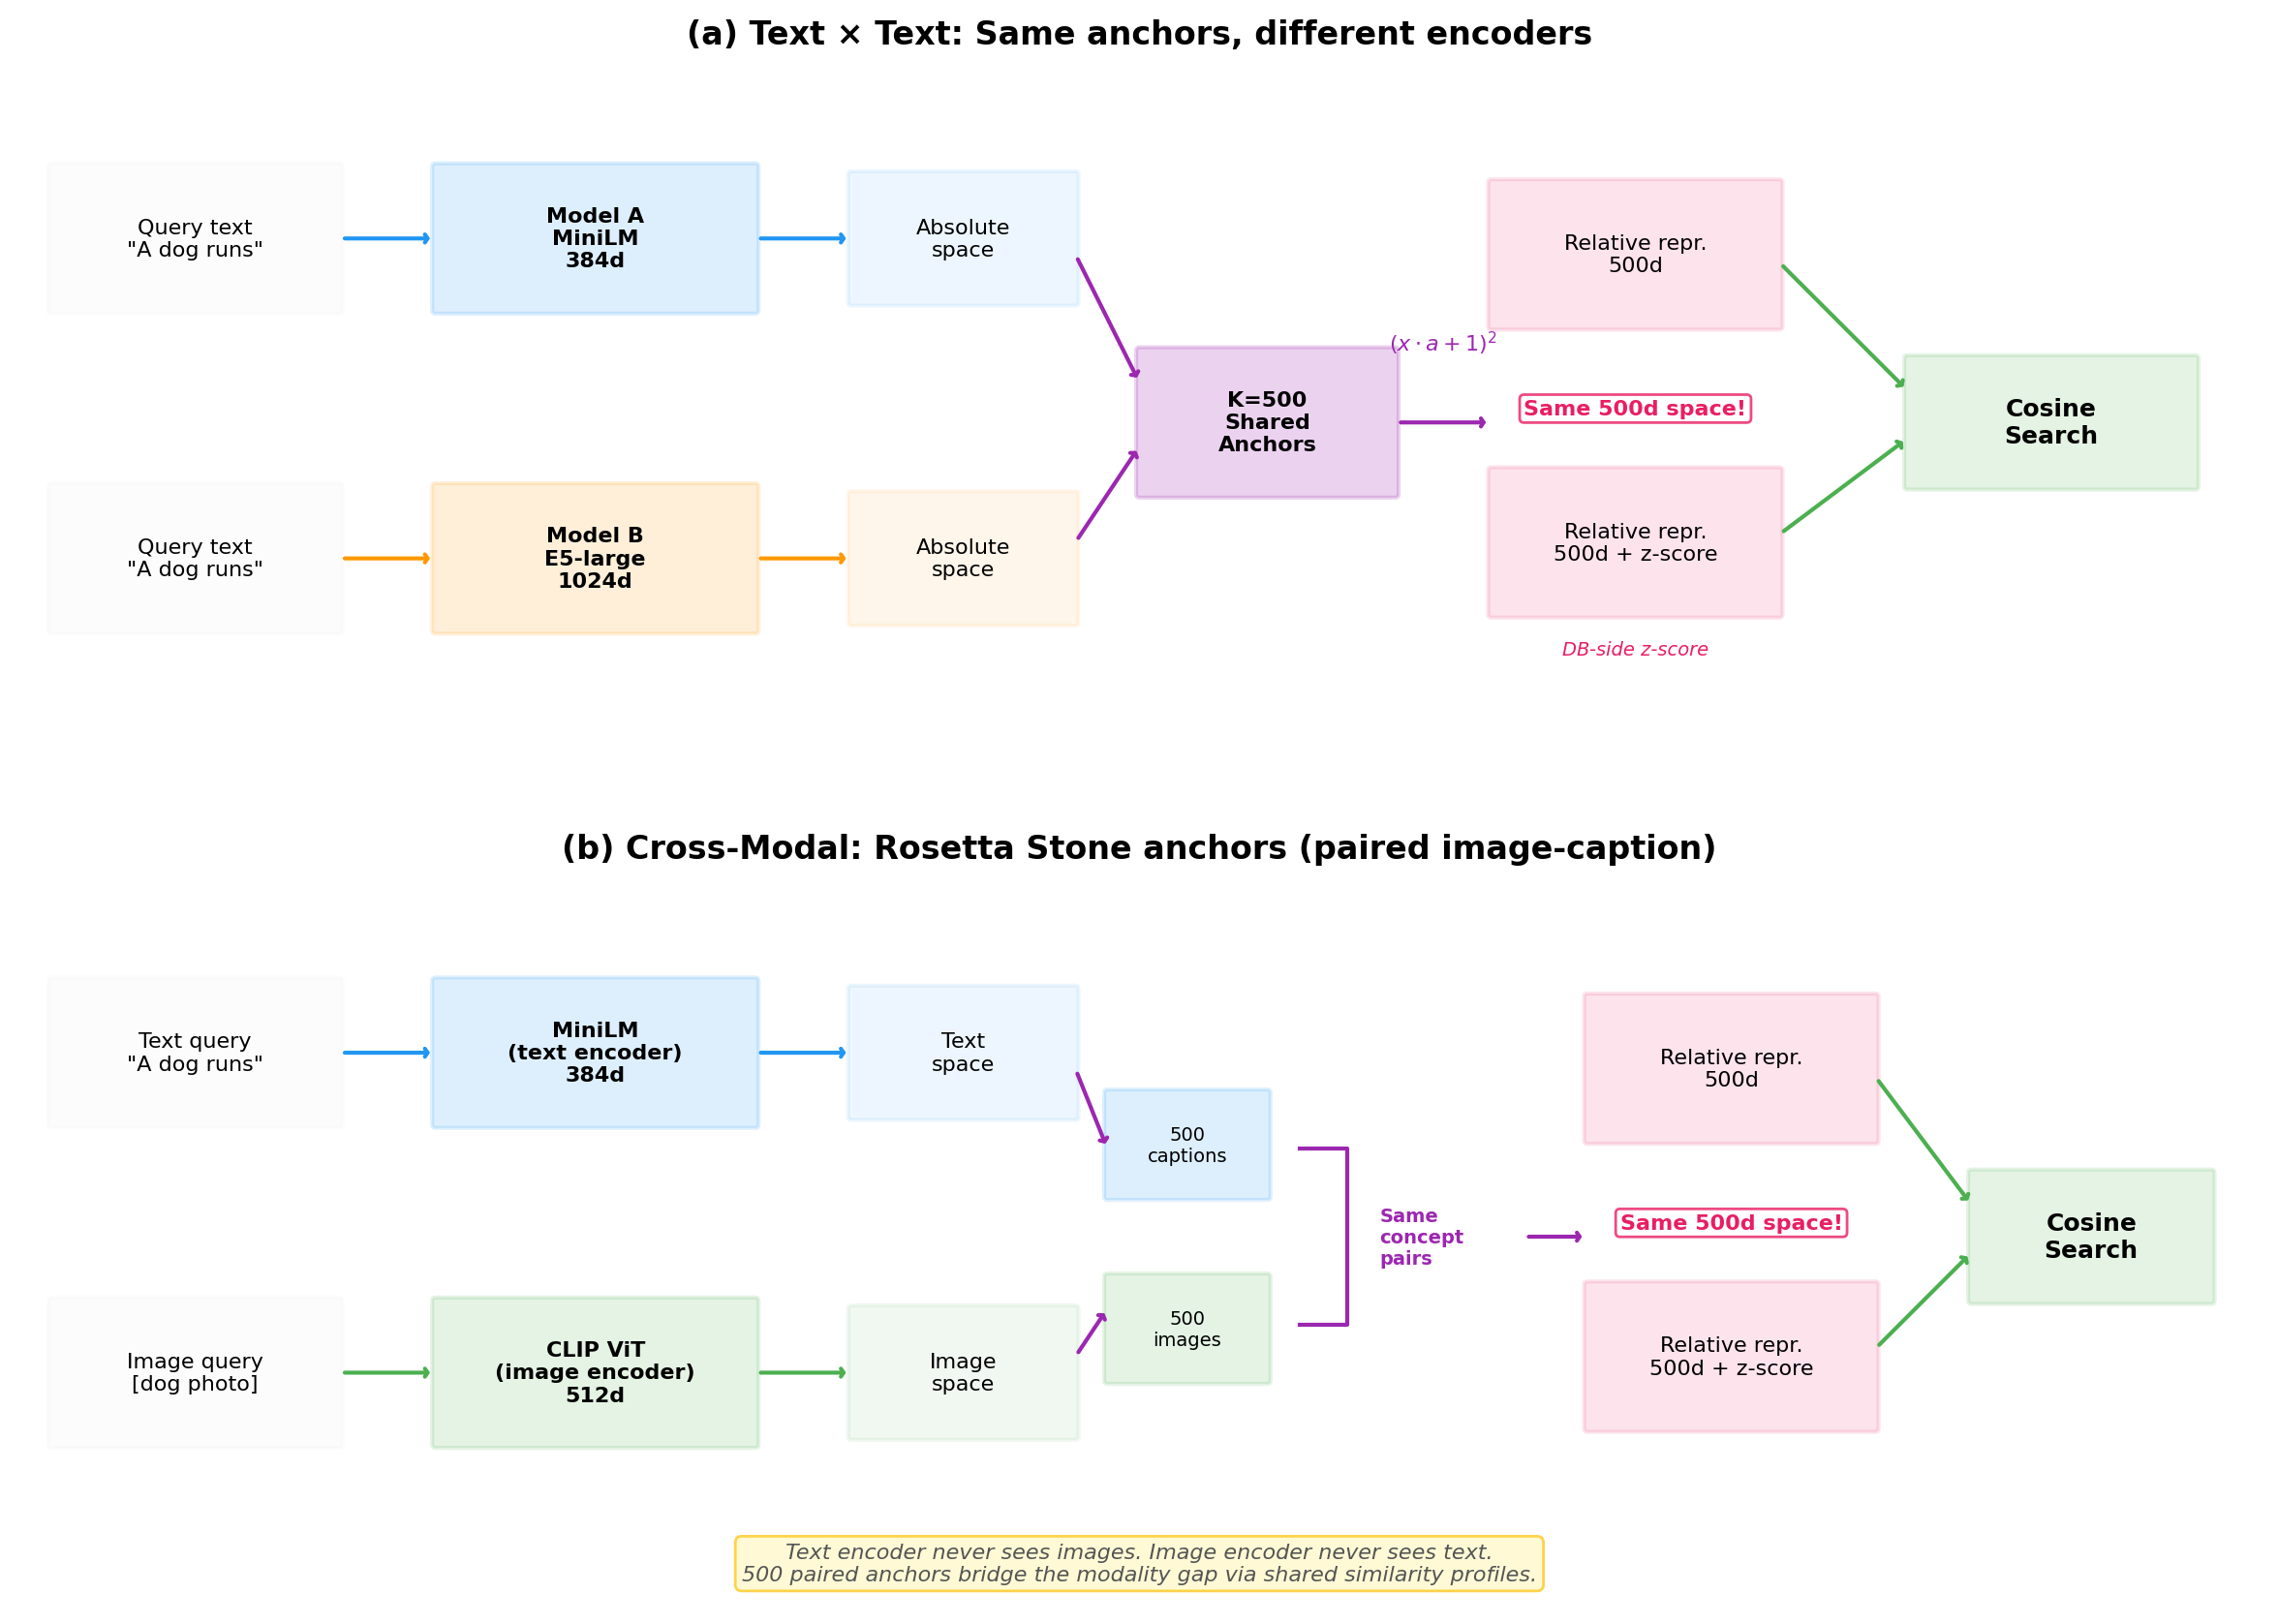
\includegraphics[width=0.75\textwidth]{figures/figure1_rat_pipeline.png}
  \caption{\textbf{RAT pipeline.} (a)~Text$\times$Text: both models encode the same anchor texts; relative representations live in a shared $K$-dimensional space regardless of original dimensions. (b)~Cross-modal: Rosetta Stone anchors provide concept-aligned (caption, image) pairs; each model encodes its own modality.}
  \label{fig:pipeline}
\end{figure}

%% ============================================================
\section{Experiments}
\label{sec:experiments}
%% ============================================================

\subsection{Setup}

\textbf{Models.} Five text encoders: MiniLM (384d, Model~A), E5-large (1024d, multilingual, Model~B), BGE-small (384d, Model~C), CLIP-text (512d, Model~D), BGE-large (1024d, Model~E). For cross-modal: CLIP ViT-B/32 image encoder (512d). Models B and E share 1024d output but differ in architecture (XLM-R vs BERT).

\textbf{Datasets.} STSBenchmark (15K sentences), AllNLI (26K sentences), COCO Karpathy (5K image-caption pairs). We sample 2,000 anchor candidates and 500 non-overlapping queries (seed=42).

\textbf{Protocol.} FPS ($K{=}500$, based on Model~A) + polynomial kernel + z-score (DB-side) + cosine kNN. Random baseline: Recall@1 = 0.2\%.

\subsection{Text-to-Text Retrieval}

\begin{table}[t]
\centering
\caption{Cross-model retrieval (Recall@1 \%) for all model pairs.}
\label{tab:text}
\begin{tabular}{@{}llcc@{}}
\toprule
Pair & Dimensions & STSBenchmark & AllNLI \\
\midrule
A$\times$C (MiniLM $\times$ BGE-small)  & 384 $\times$ 384   & 97.6 & 99.2 \\
A$\times$E (MiniLM $\times$ BGE-large)  & 384 $\times$ 1024  & 80.2 & 91.8 \\
A$\times$B (MiniLM $\times$ E5-large)   & 384 $\times$ 1024  & 83.8 & 71.8 \\
C$\times$E (BGE-small $\times$ BGE-large) & 384 $\times$ 1024 & 77.0 & 98.0 \\
B$\times$C (E5-large $\times$ BGE-small) & 1024 $\times$ 384  & 72.6 & 84.2 \\
B$\times$E (E5-large $\times$ BGE-large) & 1024 $\times$ 1024 & 55.2 & 76.4 \\
\bottomrule
\end{tabular}
\end{table}

Table~\ref{tab:text} shows results for all six model pairs. All pairs exceed 55\% on STSBenchmark and 71\% on AllNLI. Pairs involving Model~B improve markedly on AllNLI (B$\times$E +21.2pt, B$\times$C +11.6pt), reflecting AllNLI's greater semantic diversity which alleviates similarity collapse (\S\ref{sec:collapse}).

\textbf{Ablation.} On the A$\times$B pair: Random+cosine $\to$ +FPS (+23.2pt) $\to$ +poly kernel (+10.8pt) $\to$ +z-score ($\approx$0pt on this pair, but +65pt on B$\times$C).

\subsection{Anchor Efficiency: Scaling Curves}
\label{sec:scaling}

Figure~\ref{fig:scaling} compares the na\"ive baseline (random anchors + cosine) against the full RAT protocol across $K \in \{100, 200, 500, 1000\}$ on A$\times$B. \textbf{RAT at $K{=}100$ (55.0\%) surpasses random at $K{=}1000$ (48.2\%)}---proper anchor selection and kernel choice achieve higher accuracy with 10$\times$ fewer anchors. The FPS advantage is +29 to +36 points across all $K$ values. RAT saturates at $K{=}500$ (79.6\%), identifying it as the cost-optimal operating point.

\begin{figure}[t]
  \centering
  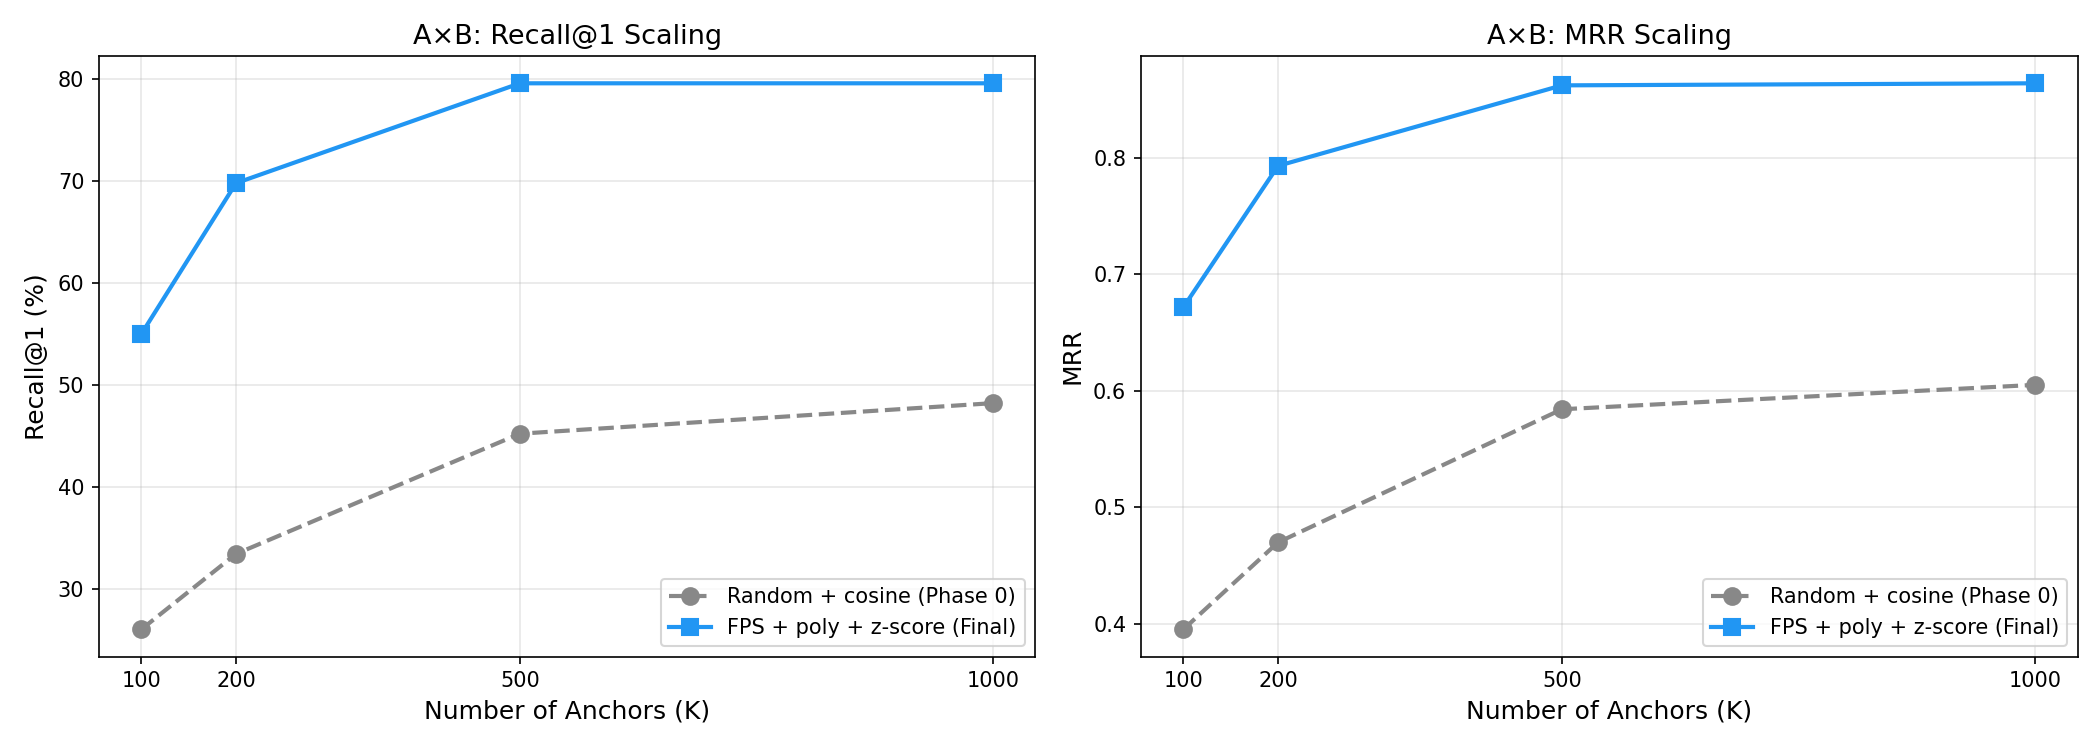
\includegraphics[width=0.7\textwidth]{figures/scaling_comparison.png}
  \caption{Scaling curves for A$\times$B: Random+cosine (dashed) vs.\ RAT protocol (solid). Left: Recall@1. Right: MRR. RAT at $K{=}100$ exceeds random at $K{=}1000$.}
  \label{fig:scaling}
\end{figure}

\subsection{Cross-Modal Retrieval}

Using 500 Rosetta Stone anchors from COCO, a text-only encoder achieves Recall@1 = 18.2\% (Image$\to$Text, with z-score) in a vision encoder's space---91$\times$ the random baseline and 29\% of CLIP's directly trained retrieval accuracy (62.0\%). Without z-score, Text$\to$Image reaches 16.4\% while Image$\to$Text drops to 3.8\%; the z-score asymmetry mirrors the text-only findings (\S\ref{sec:asymmetric}).

%% ============================================================
\section{Analysis}
\label{sec:analysis}
%% ============================================================

\subsection{Similarity Collapse}
\label{sec:collapse}

Without z-score normalization, B$\times$C achieves only 8.4\%---far below other pairs (A$\times$B: 80.6\%, A$\times$C: 98.0\%). Table~\ref{tab:collapse} traces this to anchor inter-similarity compression in Model~B's space: mean pairwise similarity of 0.72 with an effective range of only 0.33 (Figure~\ref{fig:simprofile}). This makes relative profiles nearly flat, destroying discriminability.

We term this \textbf{similarity collapse}: the failure of relative representations when the anchor similarity distribution is compressed to a narrow range. The critical diagnostic is anchor inter-similarity \emph{entropy} (Shannon entropy of the binned similarity histogram). Model~B's entropy of 1.40 is far below Model~A's 2.04.

\begin{table}[t]
\centering
\caption{Normalization methods on B$\times$C (Recall@1 \%).}
\label{tab:collapse}
\begin{tabular}{@{}lccc@{}}
\toprule
Normalization & B$\times$C & A$\times$B & A$\times$C \\
\midrule
None                   & 8.4  & 80.6 & 98.0 \\
\textbf{z-score (DB)}  & \textbf{73.4} & \textbf{81.0} & \textbf{98.2} \\
Rank transform         & 52.0 & 67.2 & 97.6 \\
Top-$k$ mask ($k{=}50$)  & 50.2 & 54.0 & 83.0 \\
Softmax ($T{=}0.1$)     & 50.2 & 34.6 & 44.8 \\
\bottomrule
\end{tabular}
\end{table}

z-score adds +65 points on B$\times$C while leaving well-spread models unharmed (+0.4 on A$\times$B). Alternative normalizations fail because they are \emph{information-destructive}: rank discards magnitude; top-$k$ zeros most entries; softmax over-sharpens. z-score uniquely preserves ordering and magnitude while correcting scale.

\begin{figure}[t]
  \centering
  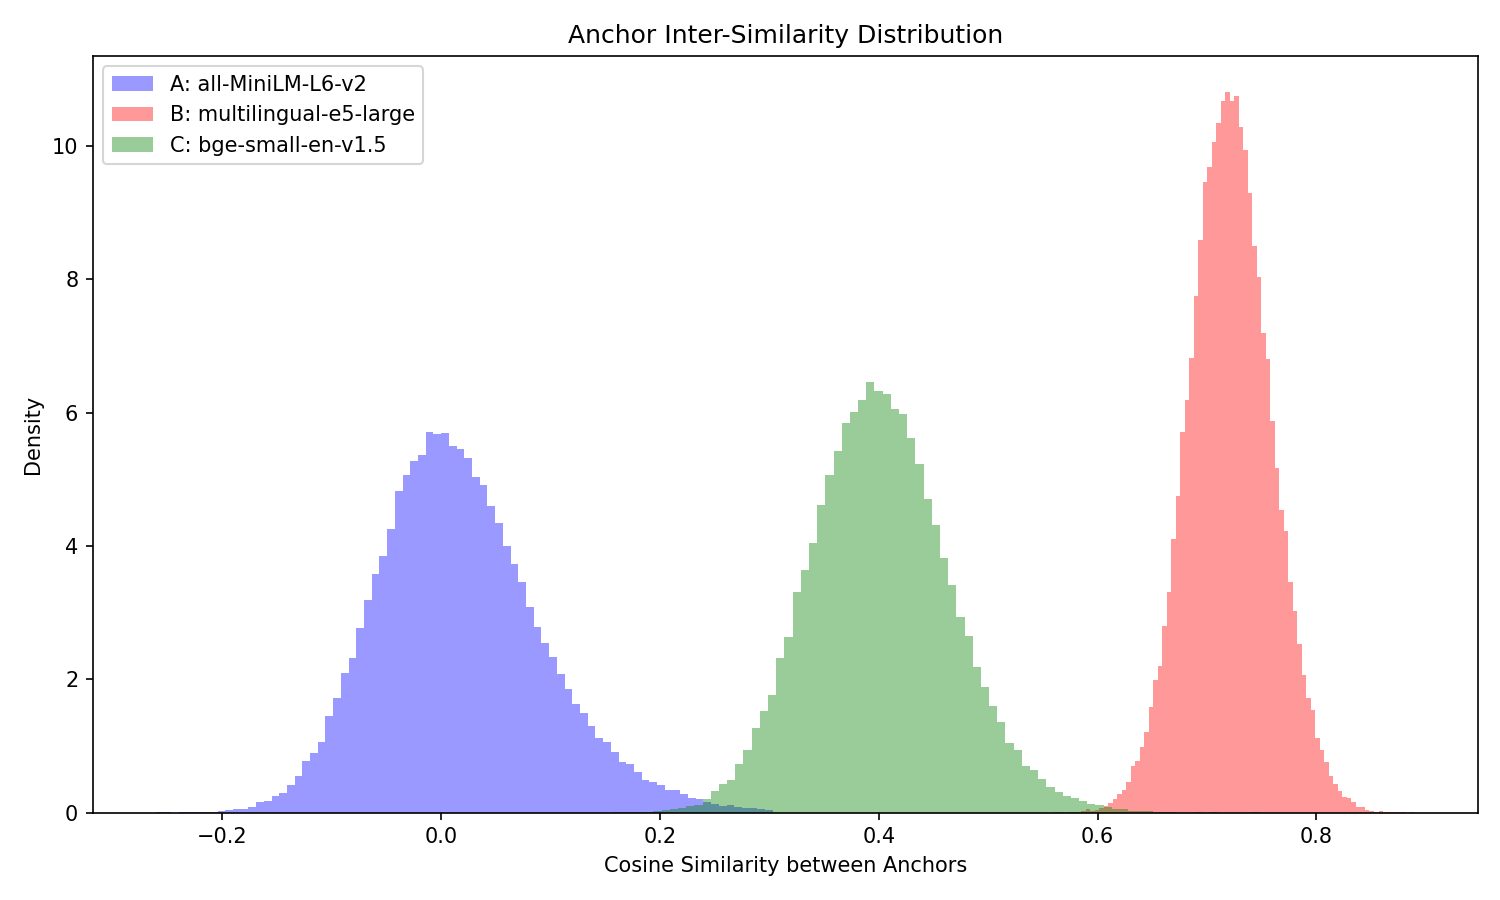
\includegraphics[width=0.7\textwidth]{figures/analysis_sim_dist.png}
  \caption{Anchor inter-similarity distributions. Model~B (E5-large) is compressed into a narrow high-similarity band, causing similarity collapse.}
  \label{fig:simprofile}
\end{figure}

\subsection{Asymmetric z-score: DB-side Sufficiency}
\label{sec:asymmetric}

\begin{table}[t]
\centering
\caption{Asymmetric z-score analysis (Recall@1 \%).}
\label{tab:asymmetric}
\begin{tabular}{@{}lcccc@{}}
\toprule
Pair / Direction & None & Query only & DB only & Both \\
\midrule
A$\times$B & 80.6 & 72.0 & \textbf{81.0} & 81.0 \\
A$\times$C & 98.0 & 90.2 & \textbf{98.2} & 98.2 \\
B$\times$C & 8.4  & 52.8 & \textbf{73.4} & 73.4 \\
\midrule
Text $\to$ Image & \textbf{16.4} & 8.2 & 15.6 & 15.6 \\
Image $\to$ Text & 3.8 & 10.0 & \textbf{18.2} & 18.2 \\
\bottomrule
\end{tabular}
\end{table}

Table~\ref{tab:asymmetric} reveals a striking pattern: \textbf{DB-only z-score exactly matches both-side z-score across all pairs and directions}. Query-side normalization is consistently harmful ($-$8 to $-$10 points on well-spread models).

DB-side normalization is effective because $n$ database vectors provide stable distributional statistics for row-wise z-scoring. A single query vector's $K$ entries yield one mean and one variance estimate; when the query model's space is already well-spread, this normalization distorts the relative magnitudes that carry discriminative signal.

\subsection{Dimensions Don't Matter: Shared Relative Structure}
\label{sec:dimensions}

Models B (E5-large) and E (BGE-large) share 1024d output but differ in architecture (XLM-R vs BERT) and training data. Their direct cosine similarity on identical texts averages $-0.02$---yet RAT achieves 55.2\% on B$\times$E, while cross-dimension A$\times$B (384d $\times$ 1024d) reaches 83.8\%. \textbf{Same-dimension B$\times$E (55\%) $<$ cross-dimension A$\times$B (84\%)}: dimensional agreement is irrelevant. RAT's Recall@1 provides a concrete operationalization of the structural convergence posited by the Platonic Representation Hypothesis \citep{huh2024platonic}, with the spectrum (55\%--98\%) offering finer granularity than a binary ``converged or not'' framing.

%% ============================================================
\section{Related Work}
\label{sec:related}
%% ============================================================

\textbf{Relative Representations.} \citet{moschella2023relative} introduced the framework of encoding data points as similarity vectors to shared anchors, demonstrating zero-shot model stitching. RAT operates within this framework: the core idea is theirs. Our contributions are (1)~showing that anchor selection matters critically (FPS achieves with 100 anchors what random requires 1,000), (2)~identifying similarity collapse as a previously uncharacterized failure mode and resolving it with z-score, and (3)~extending to cross-modal retrieval via paired anchors.

\textbf{Platonic Representation Hypothesis.} \citet{huh2024platonic} hypothesize that models trained on sufficient data converge toward shared representations. Our finding that models with zero direct correlation share relative structure (B$\times$E: 55\%) provides empirical support. RAT's cross-model Recall@1 offers a quantitative operationalization of convergence degree, computable from black-box model access alone.

\textbf{Model Stitching and Alignment.} \citet{bansal2021revisiting} train affine stitching layers; \citet{merullo2022linearly} learn linear projections for vision-language bridging; Procrustes alignment \citep{conneau2018word} fits orthogonal maps. These achieve higher precision but require paired supervision and per-pair optimization. RAT trades peak accuracy for universality: zero parameters, CPU execution, $O(1)$ cost per new model. The approaches are complementary.

%% ============================================================
\section{Limitations}
\label{sec:limitations}
%% ============================================================

\textbf{Evaluation scale.} All experiments use 500 queries from English-language datasets. Evaluation on larger benchmarks (e.g., MTEB) and multilingual settings is needed. \textbf{Cross-modal ceiling.} Recall@1 of 18.2\% is a proof of concept, not a practical system; the gap to CLIP's 62\% indicates room for improvement. \textbf{Anchor bias.} FPS in Model~A's space may not optimally cover other models' geometries; alternative bases show $\pm$2--3 point variation (Appendix). \textbf{Computational cost.} Online retrieval is $O(nK)$ per query in 500d---tractable with ANN indices (e.g., FAISS) for million-scale corpora. Offline anchor encoding is a one-time $O(nKd)$ cost. \textbf{Theory.} We provide no formal proof of why relative profiles align across models; a characterization of sufficient conditions remains open.

%% ============================================================
\section{Conclusion}
\label{sec:conclusion}
%% ============================================================

RAT translates between embedding spaces without training via three composable steps (FPS + polynomial kernel + DB-side z-score), achieving Recall@1 from 55\% to 98\% across five encoders. Key findings: similarity collapse is diagnosable and fixable (+65 points via z-score); z-score is purely a DB-side operation; and relative structure persists even when absolute coordinates are uncorrelated (cos $\approx 0$, RAT 55\%). Rosetta Stone anchors extend RAT across modalities (18.2\% Recall@1, zero visual training). Adding a new model requires only encoding shared anchors---no paired data, no gradients, no GPU.

%% ============================================================
% References
%% ============================================================

\bibliographystyle{plainnat}

\begin{thebibliography}{10}

\bibitem[Bansal et al.(2021)]{bansal2021revisiting}
Yamini Bansal, Preetum Nakkiran, and Boaz Barak.
\newblock Revisiting model stitching to compare neural representations.
\newblock In \emph{NeurIPS}, 2021.

\bibitem[Conneau et al.(2018)]{conneau2018word}
Alexis Conneau, Guillaume Lample, Marc'Aurelio Ranzato, Ludovic Denoyer, and Herv{\'e} J{\'e}gou.
\newblock Word translation without parallel data.
\newblock In \emph{ICLR}, 2018.

\bibitem[Hinton et al.(2015)]{hinton2015distilling}
Geoffrey Hinton, Oriol Vinyals, and Jeff Dean.
\newblock Distilling the knowledge in a neural network.
\newblock \emph{arXiv preprint arXiv:1503.02531}, 2015.

\bibitem[Huh et al.(2024)]{huh2024platonic}
Minyoung Huh, Brian Cheung, Tongzhou Wang, and Phillip Isola.
\newblock The platonic representation hypothesis.
\newblock In \emph{ICML}, 2024.

\bibitem[Karpathy \& Fei-Fei(2015)]{karpathy2015deep}
Andrej Karpathy and Li Fei-Fei.
\newblock Deep visual-semantic alignments for generating image descriptions.
\newblock In \emph{CVPR}, 2015.

\bibitem[Lin et al.(2014)]{lin2014microsoft}
Tsung-Yi Lin, Michael Maire, Serge Belongie, James Hays, Pietro Perona, Deva Ramanan, Piotr Doll{\'a}r, and C.~Lawrence Zitnick.
\newblock Microsoft {COCO}: Common objects in context.
\newblock In \emph{ECCV}, 2014.

\bibitem[Merullo et al.(2022)]{merullo2022linearly}
Jack Merullo, Louis Castricato, Carsten Eickhoff, and Ellie Pavlick.
\newblock Linearly mapping from image to text space.
\newblock In \emph{ICLR}, 2022.

\bibitem[Moschella et al.(2023)]{moschella2023relative}
Luca Moschella, Valentino Maiorca, Marco Fumero, Antonio Norelli, Francesco Locatello, and Emanuele Rodol{\`a}.
\newblock Relative representations enable zero-shot latent space communication.
\newblock In \emph{ICLR}, 2023.

\end{thebibliography}

%% ============================================================
% Appendix
%% ============================================================

\appendix

\section{Kernel Comparison}
\label{app:kernels}

\begin{table}[h]
\centering
\caption{Kernel function comparison on A$\times$B (Recall@1 \%, FPS $K{=}500$).}
\label{tab:kernels}
\begin{tabular}{@{}lc@{}}
\toprule
Kernel & Recall@1 \\
\midrule
Cosine ($u^\top v$) & 66.4 \\
Polynomial $(u^\top v + 1)^2$ & \textbf{77.2} \\
RBF ($\exp(-\gamma \|u-v\|^2)$) & 61.8 \\
\bottomrule
\end{tabular}
\end{table}

\section{Reproducibility}
\label{app:repro}

All experiments run on CPU (Intel, WSL2). Software: Python 3.12, sentence-transformers $\geq$2.2, transformers $\geq$4.30, scikit-learn $\geq$1.3. Random seed = 42 for all experiments. Code: \url{https://github.com/jiro-prog/rat-experiment}.

\end{document}
